% !TeX document-id = {c68f4be8-c497-43e0-82df-e9ebfbea9577}
% !TeX TXS-program:pdflatex = pdflatex -synctex=1 -interaction=nonstopmode --shell-escape %.tex
% новая команда \RNumb для вывода римских цифр
\documentclass[a4paper,12pt]{article}
\usepackage{amssymb}
\usepackage{amsmath}
\usepackage{amsthm} 
\usepackage{caption}
\usepackage{misccorr}
\usepackage[noadjust]{cite}
\usepackage{cmap} 
\usepackage[utf8]{inputenc}
\usepackage[T2A]{fontenc}
\usepackage[english, russian]{babel}
\usepackage{graphics}
\usepackage{graphicx}
\usepackage{textcomp}
\usepackage{verbatim}
\usepackage{makeidx}
\usepackage{geometry}
\usepackage{float}
\usepackage{bm}
\usepackage{esint}
\usepackage{mathtools}
\usepackage{graphicx}
\usepackage{listings}
\usepackage{courier}
\usepackage{multirow}
\usepackage{graphicx}

\lstset{basicstyle=\fontsize{10}{10}\selectfont,breaklines=true}

\newcommand{\specchapter}[1]{\chapter*{#1}\addcontentsline{toc}{chapter}{#1}}
\newcommand{\specsection}[1]{\section*{#1}\addcontentsline{toc}{section}{#1}}
\newcommand{\specsubsection}[1]{\subsection*{#1}\addcontentsline{toc}{subsection}{#1}}
\newcommand{\RNumb}[1]{\uppercase\expandafter{\romannumeral #1\relax}}
\newcommand{\jj}{\righthyphenmin=20 \justifying}


% геометрия
\geometry{pdftex, left = 2cm, right = 2cm, top = 2.5cm, bottom = 2.5cm}

\setcounter{tocdepth}{4} % фикс переноса 
\righthyphenmin = 2
\tolerance = 2048

\begin{document}
\thispagestyle{empty}

\noindent \begin{minipage}{0.15\textwidth}
	
\includegraphics[width=\linewidth]{b_logo}
\end{minipage}
\noindent\begin{minipage}{0.9\textwidth}\centering
	\textbf{Министерство науки и высшего образования Российской Федерации}\\
	\textbf{Федеральное государственное бюджетное образовательное учреждение высшего образования}\\
	\textbf{«Московский государственный технический университет имени Н.Э.~Баумана}\\
	\textbf{(национальный исследовательский университет)»}\\
	\textbf{(МГТУ им. Н.Э.~Баумана)}
\end{minipage}

\noindent\rule{18cm}{3pt}
\newline\newline
\noindent ФАКУЛЬТЕТ $\underline{\text{«Информатика и системы управления»}}$ \newline\newline
\noindent КАФЕДРА $\underline{\text{«Компьютерные системы и сети»}}$\newline\newline
\noindent НАПРАВЛЕНИЕ ПОДГОТОВКИ $\underline{\text{«09.03.04 Программная инженерия»}}$\newline\newline\newline\newline\newline


\begin{center}
	\noindent\begin{minipage}{1.3\textwidth}\centering
	\Large\textbf{  ОТЧЕТ }\newline
	\textbf{по лабораторной работе №1}\newline\newline
	\end{minipage}
\end{center}

\noindent\textbf{Название:} $\underline{\text{Синхронные одноступенчатые триггеры со статическим и динамическим}}$\newline
\noindent$\underline{\text{управлением записью}}$\newline\newline
\noindent\textbf{Дисциплина:} $\underline{\text{Архитектура ЭВМ}}$\newline\newline\newline\newline\newline

\begin{center}
	\begin{tabular}{ccccc}
		Студент: & $\underline{\text{ИУ7-43Б}}$ & $\underline{\text{~~~~~~~~~~~}}$ & $\underline{\text{31.03.2020}}$ & $\underline{\text{А. В. Романов}}$ \\
		 & \footnotesize группа & \footnotesize подпись & \footnotesize дата  & \footnotesize (И. О. Фамилия) \\
		  &  &  &  & \\
		Преподаватель: & \textbf{} & $\underline{\text{~~~~~~~~~~~}}$ & $\underline{\text{~~~~~~~~~~~~}}$ & $\underline{\text{А. Ю. Попов}}$ \\
		&  & \footnotesize подпись & \footnotesize дата  & \footnotesize (И. О. Фамилия) \\
	\end{tabular}
\end{center}


\begin{center}
	\vfill
	Москва~---~\the\year
~г.
\end{center}
\clearpage


\section{Цель работы} Изучить схемы асихнроного RS-тригера, который является запоминающей ячейкой всех типов триггеров, синхронных RS- и D-триггеров со статическим управлением записью и DV-триггера с динамическим управлением записью.

\section{Асинхроный RS-тригер с инверсными входами в статическом режиме}\label{chap:rs-trigger}

\begin{center}
	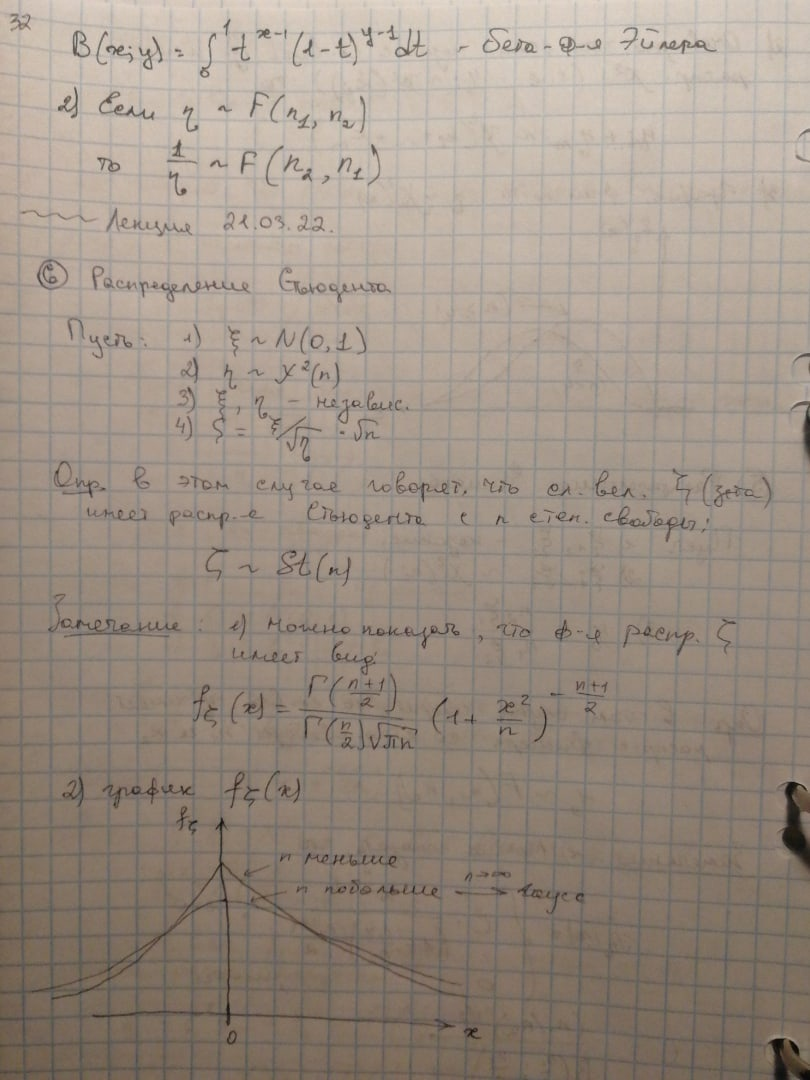
\includegraphics[scale=1]{../screens/1.jpg} \newline\newline
	Таблица переходов: 
	
	\begin{center}
		\begin{tabular}{ | l | l | l | l | l | p{1cm} |}
			\hline
			$S$ & $R$ & $Q_{n}$ & $Q_{n + 1}$ & Режим\\ \hline
			0 & 0 & 0 & 0 & {\multirow{2}{*}{Хранение}} \\ 
			0 & 0 & 1 & 1 & \\ \hline
			
			0 & 1 & 0 & 0 & {\multirow{2}{*}{0}} \\ 
			0 & 1 & 1 & 0 & \\ \hline
			
			1 & 0 & 0 & 1 & {\multirow{2}{*}{1}} \\ 
			1 & 0 & 1 & 1 &  \\ \hline
			
			1 & 1 & 0 & X & {\multirow{2}{*}{Запрещённое состояние}}  \\
			1 & 1 & 1 & X &  \\
			\hline
		\end{tabular}
	\end{center}
\end{center}

\noindent Можно заметить, что $S$ устанавливает тригер в состояние единицы, а $R$ устанавливает в состояние нуля. Одновременая подача $S$ и $R$ запрещена.\newline

\noindent Файл: 1.ms12

\section{Синхроный RS-тригер в статическом режиме}

\begin{center}
	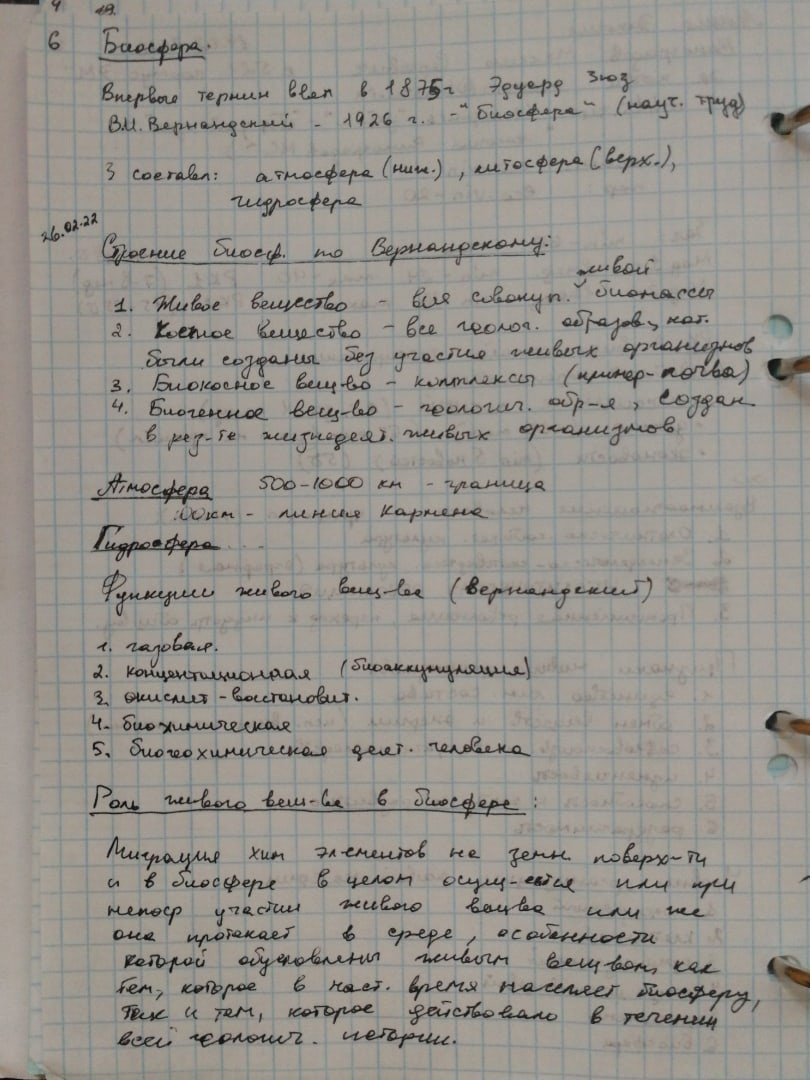
\includegraphics[scale=1]{../screens/2.jpg} \newline\newline
	Таблица переходов: 
	
	\begin{center}
		\begin{tabular}{ | l | l | l | l | l | l | p{1cm} |}
			\hline
			$C$ & $S$ & $R$ & $Q_{n}$ & $Q_{n + 1}$ & Режим\\ \hline
			0 & * & * & 0 & 0 & {\multirow{2}{*}{Хранение}} \\ 
			0 & * & * & 1 & 1 & \\ 
			1 & 0 & 0 & 0 & 0 &  \\ 
			1 & 0 & 0 & 1 & 1 &  \\ \hline
			
			1 & 0 & 1 & 0 & 0 & {\multirow{2}{*}{0}} \\ 
			1 & 0 & 1 & 1 & 0 & \\ \hline
			
			1 & 1 & 0 & 0 & 1 & {\multirow{2}{*}{1}} \\ 
			1 & 1 & 0 & 1 & 1 & \\ \hline
			
			1 & 1 & 1 & 0 & X & {\multirow{2}{*}{Запрещённое состояние}} \\ 
			1 & 1 & 1 & 1 & X & \\
			\hline
		\end{tabular}
	\end{center}
\end{center}

\noindent Вход $C$ позволяет внести контроль над сигналом, входящим в триггер.\newline

\noindent Файл: 2.ms12

\section{D-триггер в статическом режиме}


\begin{center}
	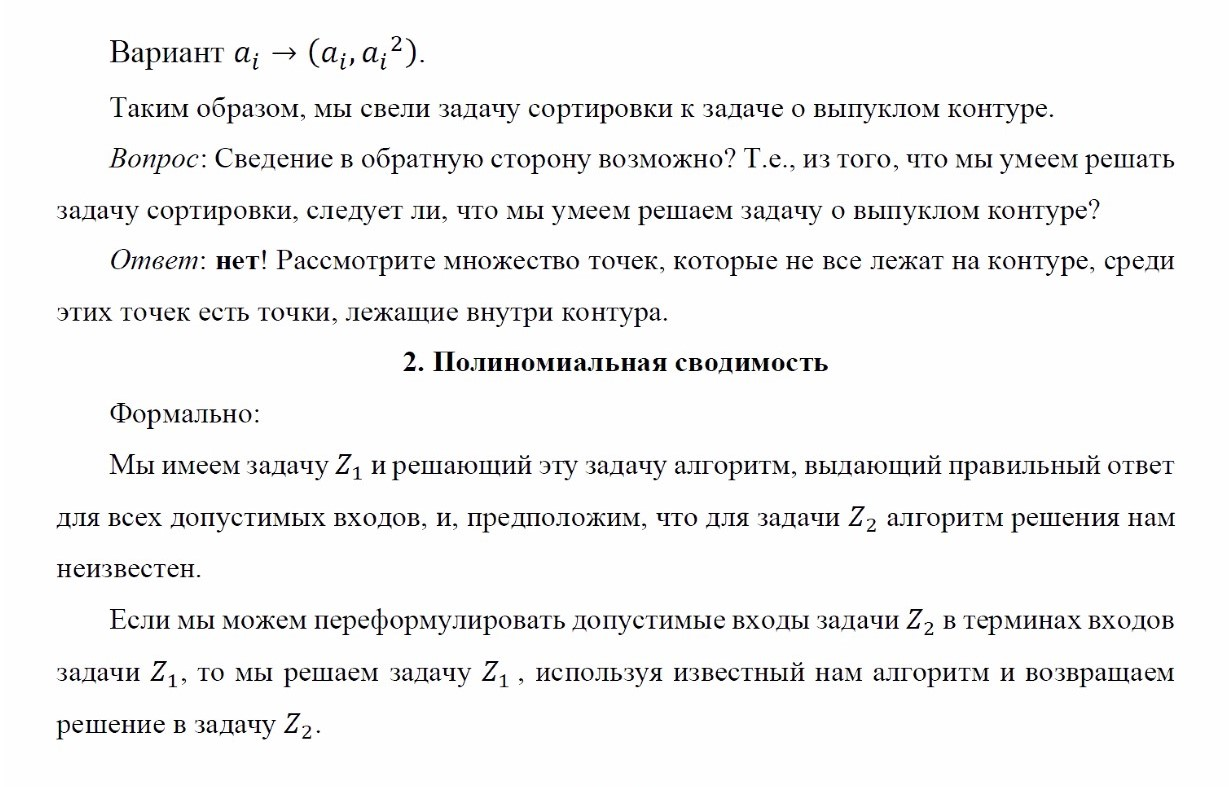
\includegraphics[scale=1]{../screens/3.jpg} \newline\newline
	Таблица переходов: 
	
	\begin{center}
		\begin{tabular}{ | l | l | l | l | l | p{1cm} |}
			\hline
			$C$ & $D$ & $Q_{n}$ & $Q_{n + 1}$ & Режим\\ \hline
			0 & * & 0 & 0 & {\multirow{2}{*}{Хранение}} \\ 
			0 & * & 1 & 1 & \\ \hline
			
			1 & 0 & 0 & 0 & {\multirow{2}{*}{0}} \\ 
			1 & 0 & 1 & 0 & \\ \hline
			
			1 & 1 & 0 & 1 & {\multirow{2}{*}{1}} \\ 
			1 & 1 & 1 & 1 & \\ 
			\hline
		\end{tabular}
	\end{center}
\end{center}

\noindent Сигналы на входе D до переключения и на выходе после переключения совпадают.\newline

\noindent Файл: 3.ms12

\clearpage
\section{Синхронный D-триггер с динамическим управлением}

\begin{center}
	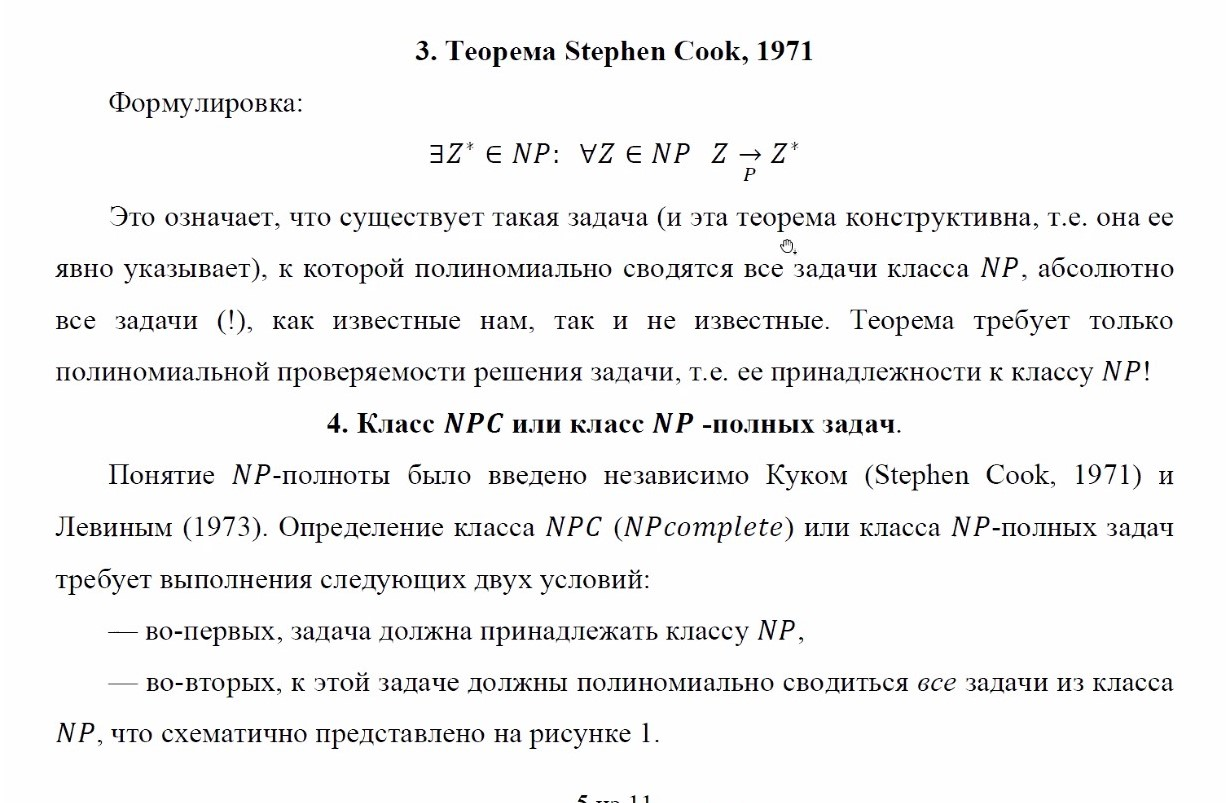
\includegraphics[scale=1.3]{../screens/4.jpg} \newline\newline
	Таблица переходов: 
	
	\begin{center}
		\begin{tabular}{ | l | l | l | p{1cm} |}
			\hline
			$D$ & $C$ & $Q$ \\ \hline
			0 & 0 & {\multirow{2}{*}{0}} \\
			0 & 1 & \\ \hline
			
			1 & 0 & {\multirow{2}{*}{1}} \\
			1 & 1 & \\ \hline
			
			X & X & Хранение \\ 
			\hline
		\end{tabular}
	\end{center}
\end{center}

\noindent Прием информационных сигналов и передача на выход принятой информации выполняются в момент изменения синхросигнала на $C$-входе из 0 в I или из I в 0, т.е. особенностью синхронных триггеров с динамическим управлением является перепад синхросигнала. \newline

\noindent Файл: 4.ms12

\clearpage
\section{Синхронный DV-триггер с динамическим управлением}

\begin{center}
	
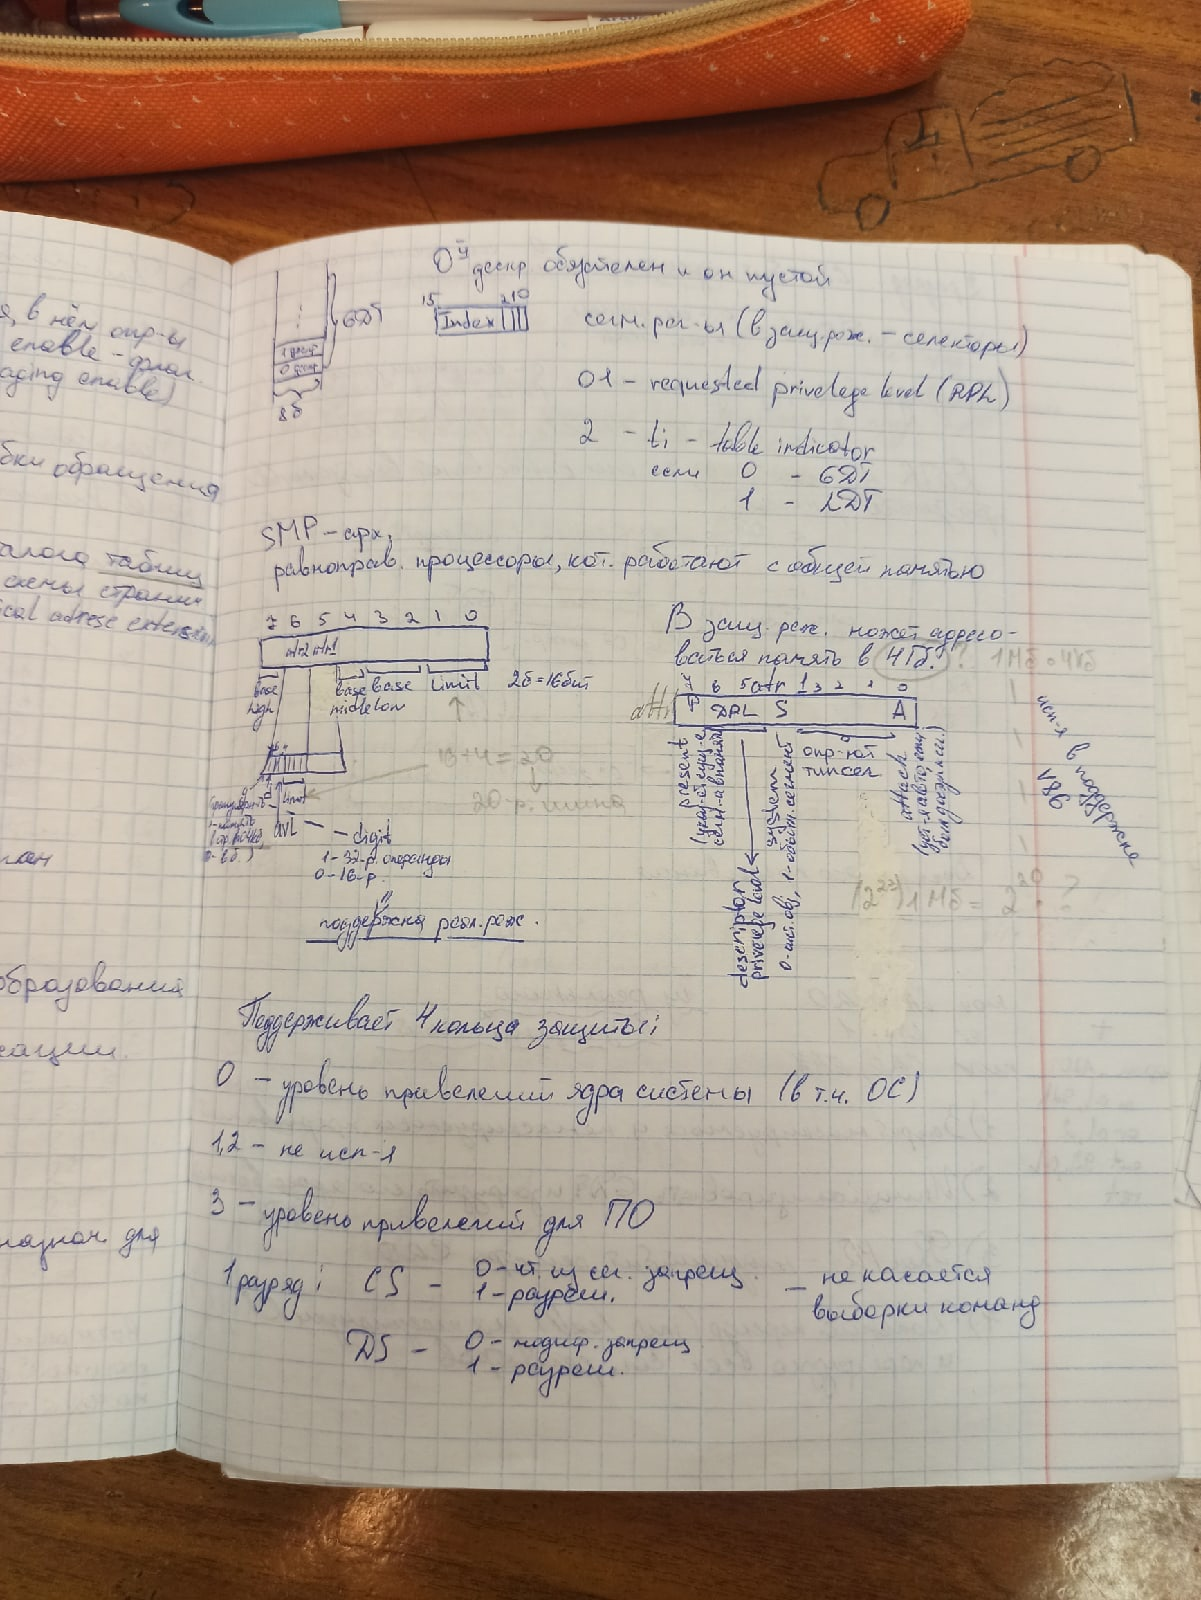
\includegraphics[scale=1]{../screens/5.jpg} \newline\newline
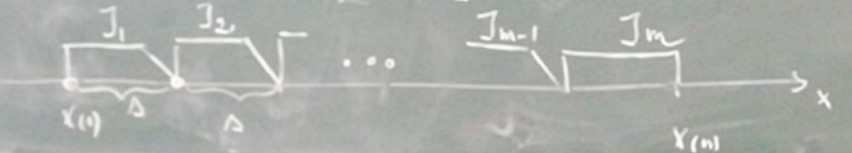
\includegraphics[scale=1]{../screens/5_1.jpg} \newline\newline

\end{center}

\noindent При $C = 0$ имеем $Q_{t} = Q_{t - 1}$ (сохраняется предыдущее состояние). При $C = 1 $ и $V = 0$ триггер сохраняет предыдущее внутреннее состояние. При $C = V = 1$ триггер принимает сигнал на входе $D$.\newline

\noindent Файл: 5.ms12


\section{DV-триггер, включенный по схеме TV-триггера}

\begin{center}
	
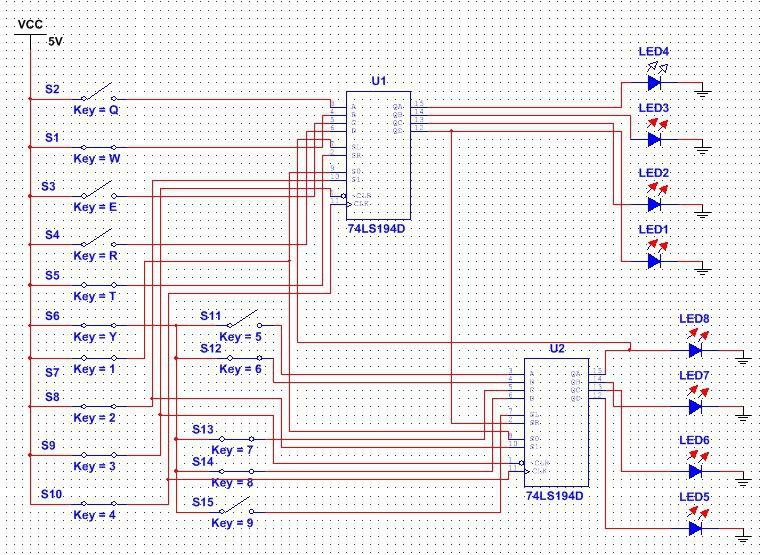
\includegraphics[scale=1.2]{../screens/6.jpg} \newline\newline
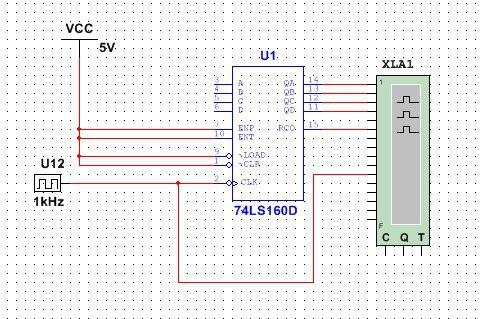
\includegraphics[scale=1]{../screens/6_1.jpg} \newline\newline

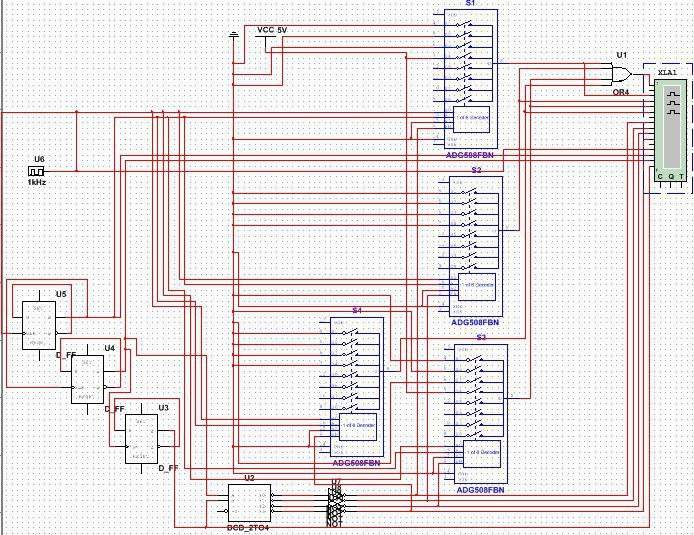
\includegraphics[scale=1]{../screens/7.jpg} \newline\newline
 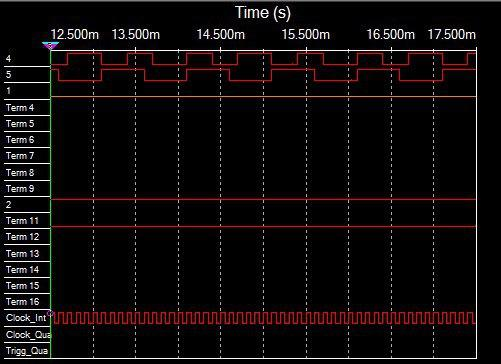
\includegraphics[scale=1]{../screens/7_1.jpg} \newline\newline
 
\end{center}
 
\noindent \textbf{Асинхронный T-триггер} переходит в противоположное состояние каждый раз при подаче на $T$-вход единичного сигнала. $T$-триггер реализует счет по модулю 2: $Q_{n + 1} = T \oplus Q_{n}$. \textbf{Синхронный Т-триггер} имеет вход $C$ и вход $T$. Синхронный $T$-триггер переключается в противоположное состояние сигналом С, если на счетном входе Т действует единичный сигнал.\newline

\noindent Файлы: 6.ms и 7.ms

\clearpage
\section{Вывод}

\noindent При выполнении этой лабораторной работы я познакомился с принципом работы, минусами и плюсами, нуждой в какой-либо ситуации и схемами различных триггеров.

\section{Контрольные вопросы}

\noindent\textbf{1.} Что называется триггером?\newline

\noindent\textbf{Триггер} -- запоминающее устройство, имеющие два устойчивых состояния, которые кодируются двоичными цифрами $0$ и $1$\newline

\noindent\textbf{2.} Какова структурная схема триггера? \newline

\noindent Структурная схема триггера состоит из \textbf{запоминающей ячейки} и \textbf{схемы управления}.\newline

\noindent\textbf{3.} По каким основным признакам классифицируют триггеры?\newline

\noindent\textbf{1) }По способу организации логических связей, т.е. по виду логического уравнения, характеризующего состояние входов и выходов триггера в момент времени $t_{n}$ до его срабатывания и в момент $t_{n+1}$ после его срабатывания, различают триггеры: 

\textbf{а) } с раздельной установкой состояний 0 и 1 ($RS$-триггеры)

\textbf{б) } со счетным входом ($Т$-триггеры)

\textbf{в) } универсальные с раздельной установкой состояний 0 и 1 ($JK$-триггеры)

\textbf{г) } с приемом информации по одному входу ($D$ триггеры)

\textbf{д) } универсальные с управляемым приемом информации по одному входу ($DV$-триггеры)

\textbf{е) } комбинированные (например, $RST$-, $JKRS$, $DRS$-триггеры) и т.д.\newline

\noindent\textbf{2) }По способу запаси информации различают триггеры: 

\textbf{а) } асинхронные (не синхронизируемые).

\textbf{б) } синхронные (синхронизируемые), или тактируемые.\newline

\noindent\textbf{3) }По способу синхронизации различают триггеры: синхронные со статическим управлением записью; синхронные с динамическим управлением записью. \newline

\noindent\textbf{4) }По способу передачи информации с входов на выход различают триггеры о одноступенчатым и двухступенчатым запоминанием информации.\newline

\noindent\textbf{4.} Каково функциональное назначение входов триггеров?\newline

\noindent\textbf{S-вход} -- вход для раздельной установки триггера в состояние "1".\newline
\noindent\textbf{R-вход} -- вход для раздельной установки триггера в состояние "0".\newline
\noindent\textbf{J-вход} -- вход для установки состояния "1" в универсальном JK-триггере.\newline
\noindent\textbf{K-вход} -- вход для установки состояния "0" в универсальном JK-триггере.\newline
\noindent\textbf{D-вход} -- информационный вход для установки триггера в состояния "1" или "0".\newline
\noindent\textbf{V-вход} -- подготовительный управляющий вход для разрешения приема информации.\newline
\noindent\textbf{C-вход} -- исполнительный управляющий вход для осуществления приема информации, вход синхронизации.\newline

\noindent\textbf{5.} Что такое асинхронный и синхронный триггеры?\newline

\noindent\textbf{Ассинхронный RS-триггер} -- простейший триггер, использующийся как запоминающая ячейка.\newline
\noindent\textbf{Синхроный RS-триггер} -- имеет два информационных входа $R$ и $S$ и вход синхронизации $C$.\newline

\noindent\textbf{6.} Что такое таблица переходов?\newline

\noindent\textbf{Таблица переходов} -- отображает зависимость выходного сигнала триггера в момент времени $t_{n + 1}$ от входных сигналов и от состояния триггера в предыдущий момент времени $t_{n}$\newline

\noindent\textbf{7.} Как работает асинхронный $RS$-триггер?\newline

\noindent При $S = 0$ и $R = I$ триггер устанавливается в состояние 0, а при $S = 1$ и $R = 0$ - в состояние 1. Если $S = 0$ и $R = 0$, то в триггере сохраняется предыдущее внутреннее состояние. 
При $S = R = 1$ состояние триггера является неопределенным (после снятия входных сигналов $S$ и $R$). Такая комбинация входных сигналов $S = R = 1$ является недопустимой (запрещенной). Для нормальной работы триггера необходимо выполнение запрещающего условия $SR = 0$.\newline

\noindent\textbf{8.} Как работает синхронный $RS$-триггер? Какова его таблица переходов? \newline

\noindent Как и все синхронные триггеры, \textbf{синхронный RS-триггер} при $C = 0$ сохраняет предыдущее внутреннее состояние, т.е. $Q_{n + 1} = Q_{n}$. Сигналы по входам $S$ и $R$ переключают синхронный $RS$-триггер только с поступлением импульса на вход синхронизации $С$. При $С = 1$ синхронный триггер переключается как асинхронный. Одновременная подача сигналов $С = S = R = 1$ запрещена. При $S = R = 0$ триггер не изменяет своего состояния.\newline

\noindent Таблица переходов находится в разделе RS-триггеров.\newline

\noindent\textbf{9.} Что такое $D$-триггер? \newline

\noindent\textbf{Синхронный D-триггер} -- имеет один информационный вход $D$, состояние которого с каждым синхронизирующим импульсом передается на выход, т.е. выходные сигналы представляют собой задержанные входные сигналы. Поэтому $D$-триггер -- элемент задержки входных сигналов на один такт.\newline

\noindent\textbf{10.} Объясните работу синхронного $D$-триггера.\newline

\noindent Схему \textbf{синхронного D-триггера} можно получить из схемы синхронного $RS$-триггера, подавая сигнал $D$ на вход $S$, а сигнал $D-$, т.е. с выхода инвертора сигнала $D$, на вход $R$. В результате на входах $RS$-триггера возможны только наборы сигналов $SR = 01$ при $D = 0$ или $SR = 10$ при $D = 1$, что соответствует записи в триггер логического 0 или 1. Путем логических преобразований инвертор можно исключить и получить схему синхронного $D$-триггера. Синхронный $D$-триггер имеет один информационный вход $D$, состояние которого с каждым синхронизирующим импульсом передается на выход, т.е. выходные сигналы представляют собой задержанные входные сигналы.\newline

\noindent\textbf{11.} Что такое $DV$–триггер? \newline

\noindent\textbf{Синхронный DV-триггер} -- имеет один информационный вход $D$ и один подготовительный разрешающий вход $V$ для разрешения приема информации.\newline

\noindent\textbf{12.} Объясните работу $DV$-триггера. \newline

\noindent\textbf{DV-триггер}, при $C = 0$, как и синхронные триггеры всех типов, сохраняет предыдущее внутреннее состояние, т.е. $Q_{n + 1} = Q_{n}$. При $C = 1$ и при наличии сигнала $V = 1$ разрешения приема информации $DV$-триггер принимает информационный сигнал, действующий на входе $D$, т.е. работает как асинхронный $DV$-триггер. При $C = 1$ и $V = 0$ $DV$-триггер сохраняет предыдущее внутреннее состояние, т.е. $Q_{n + 1} = Q_{n}$\newline

\noindent\textbf{13.} Что такое $T$-триггер? Какова его таблица переходов? \newline

\noindent\textbf{Т-триггер} имеет один информационный вход $T$, называемый счетным входом. Асинхронный $T$-триггер переходит в противоположное состояние каждый раз при подаче на $T$-вход единичного сигнала. Таким образом $T$-триггер реализует счет по модулю 2: $Q_{t} = T_{t - 1} \oplus Q_{t - 1}$.Синхронный $Т$-триггер имеет вход $C$ и вход $T$. Синхронный $T$-триггер переключается в противоположное состояние сигналом $C$, если на счетном входе $T$ действует сигнал логической 1.\newline

\noindent\textbf{14.} Объясните работу схемы синхронного $RS$-триггера со статическим управлением. \newline

\noindent При $C = 0$ триггеры переходят в режим хранения, запоминая последнее состояние.\newline

\noindent\textbf{15.} Какова характерная особенность переключения синхронных триггеров с динамическим управлением записью? \newline

\noindent Характерной особенностью синхронных триггеров с динамическим управлением записью является то, что приём информационных сигналов и передача на выход принятой информации выполняются в момент изменения синхросигнала на $C$-входе из 0 в 1 или из 1 в 0, т.е. перепадом синхросигнала.\newline

\noindent\textbf{16.} Как работает схема синхронного $D$-триггера с динамическим управлением записью на основе трех RS -триггеров? \newline

\noindent Триггер имеет асинхронные входы $S_{a}$ и $R_{a}$ начальной установки в состояния 1 и 0. Если схему $D$-триггера дополнить входом $V$, то получим структуру $DV$-триггера. Временные диаграмы $D$-триггера соответствуют временным диаграммам $DV$-триггера при $V = 1$\newline

\clearpage
\noindent\textbf{17.} Составьте временные диаграммы работы синхронного $D$-триггера с динамическим управлением записью. \newline

\noindent Временные диаграмы находятся в разделе $D$-триггеры.\newline

\noindent\textbf{18.} Какова структура и принцип действия синхронного $DV$-триггера с динамическим управлением записью? \newline

\noindent Синхронный DV-триггер имеет один информационный вход D и один подготовительный разрешающий вход V для разрешения приема информации. $$Q_{t} = DV + VQ_{t - 1} = DVC + (V + C)Q_{t - 1}$$

\noindent При $C = 0$ $DV$-триггер, как и синхронные триггеры всех типов, сохраняет предыдущее внутреннее состояние.\newline При $C = 1$ и при наличии сигнала $V = 1$ разрешения приема информации $DV$-триггер принимает информационный сигнал, действующий на входе $D$.\newline При $C = 1$ и $V = 0$ $DV$-триггер сохраняет предыдущее внутреннее состояние.\newline

\noindent\textbf{19.} Составьте временные диаграммы синхронного DV-триггера. \newline

\noindent Временные диаграммы находятся в разделе $DV$-триггеры.\newline

\noindent\textbf{20.} Объясните режимы работы $D$-триггера. \newline

\noindent\textbf{Синхронный D-триггер} -- имеет один информационный вход $D$, состояние которого с каждым синхронизирующим импульсом передается на выход, т.е. выходные сигналы представляют собой задержанные входные сигналы.

\end{document}